\documentclass[sigconf]{acmart}
\usepackage{enumerate}

\AtBeginDocument{%
	\providecommand\BibTeX{%
		{%
			Bib\TeX
		}
	}
}
\setcopyright{acmlicensed}
\copyrightyear{2018}
\acmYear{2018}
\acmDOI{XXXXXXX.XXXXXXX}
\acmConference[Conference acronym 'XX]{Make sure to enter the correct conference title from your rights confirmation email}{June 03--05, 2018}{Woodstock, NY}
\acmISBN{978-1-4503-XXXX-X/18/06}

\begin{document}

\title{Title}

\author{San Zhang\textsuperscript{\#}}
\affiliation{%
	\institution{Department/College/School/Faculty/\\Institute/... A, University A}
	\streetaddress{Street A}
	\city{City A}
	\country{Country/Region A}
}
\email{sanzhang@gmail.com}
\orcid{0000-0000-0000-0003}

\author{Si Li\textsuperscript{\#}}
\affiliation{%
	\institution{Department/College/School/Faculty/\\Institute/... B, University B}
	\streetaddress{Street B}
	\city{City B}
	\country{Country/Region B}
}
\email{sili@gmail.com}
\orcid{0000-0000-0000-0004}

\author{Wu Wang}
\affiliation{%
	\institution{Department/College/School/Faculty/\\Institute/... C, University C}
	\streetaddress{Street C}
	\city{City C}
	\country{Country/Region C}
}
\email{wuwang@gmail.com}
\orcid{0000-0000-0000-0005}

\author{Liu Zhao*}
\affiliation{%
	\institution{Department/College/School/Faculty/\\Institute/... D, University D}
	\streetaddress{Street D}
	\city{City D}
	\country{Country/Region D}
}
\email{liuzhao@gmail.com}
\orcid{0000-0000-0000-0006}

\author{Qi Sun*}
\affiliation{%
	\institution{Department/College/School/Faculty/\\Institute/... E, University E}
	\streetaddress{Street E}
	\city{City E}
	\country{Country/Region E}
}
\email{qisun@gmail.com}
\orcid{0000-0000-0000-0007}

\renewcommand{\shortauthors}{Zhang S, Li S, Wang W, et al. }

\begin{abstract}
	This is a one-paper-multiple-typesetting-styles template. With this template, users can easily switch to different LaTeX typesetting styles while maintaining up-to-date content. For example, in case a paper is unfortunately rejected without being reviewed, users can switch to a better journal or conference immediately or even directly. We hope all papers can be accepted in a suitable and satisfying place. 
\end{abstract}

\keywords{LaTeX, Typesetting}

\received{3 November 2024}
\received[revised]{26 November 2024}
\received[accepted]{10 February 2025}

\maketitle

\renewcommand{\thefootnote}{}
\footnotetext{* Theses are the corresponding authors. }

%%%%%%%%%%%%%%%%%%%%%%%%%%%%%%%%%%%%%%%
\section{Introduction}
\label{sec:1}

This is the introduction. See links \cite{linkEnglish, linkChinese, linkScript} for more information. This is the introduction. See links \cite{linkEnglish, linkChinese, linkScript} for more information. This is the introduction. See links \cite{linkEnglish, linkChinese, linkScript} for more information. This is the introduction. See links \cite{linkEnglish, linkChinese, linkScript} for more information. This is the introduction. See links \cite{linkEnglish, linkChinese, linkScript} for more information. This is the introduction. See links \cite{linkEnglish, linkChinese, linkScript} for more information. This is the introduction. See links \cite{linkEnglish, linkChinese, linkScript} for more information. This is the introduction. See links \cite{linkEnglish, linkChinese, linkScript} for more information. This is the introduction. See links \cite{linkEnglish, linkChinese, linkScript} for more information. This is the introduction. See links \cite{linkEnglish, linkChinese, linkScript} for more information. 

The remaining sections are structured as follows. Section~\ref{sec:2} is the related work. Section~\ref{sec:3} is the methodology. Section~\ref{sec:4} presents the experiments. Section~\ref{sec:5} presents the experimental results and discussion. Section~\ref{sec:6} is the conclusion, which concludes the whole work. Some possible future research directions are proposed. 
\section{Related Work}
\label{sec:2}

This is the related work. This is the related work. This is the related work. This is the related work. This is the related work. This is the related work. This is the related work. This is the related work. This is the related work. This is the related work. 
\section{Methodology}
\label{sec:3}

This is the methodology. This is the methodology. This is the methodology. This is the methodology. This is the methodology. This is the methodology. This is the methodology. This is the methodology. This is the methodology. This is the methodology. 
\section{Experiments}
\label{sec:4}

These are the experiments. These are the experiments. These are the experiments. These are the experiments. These are the experiments. These are the experiments. These are the experiments. These are the experiments. These are the experiments. These are the experiments. 
\section{Results and Discussion} 
\label{sec:5}

These are the results and discussion. These are the results and discussion. These are the results and discussion. These are the results and discussion. These are the results and discussion. These are the results and discussion. These are the results and discussion. These are the results and discussion. These are the results and discussion. These are the results and discussion. 

\subsection{Experimental results}

An example figure is shown in Fig.~\ref{fig:tree}. 

\begin{figure*}
	\centerline{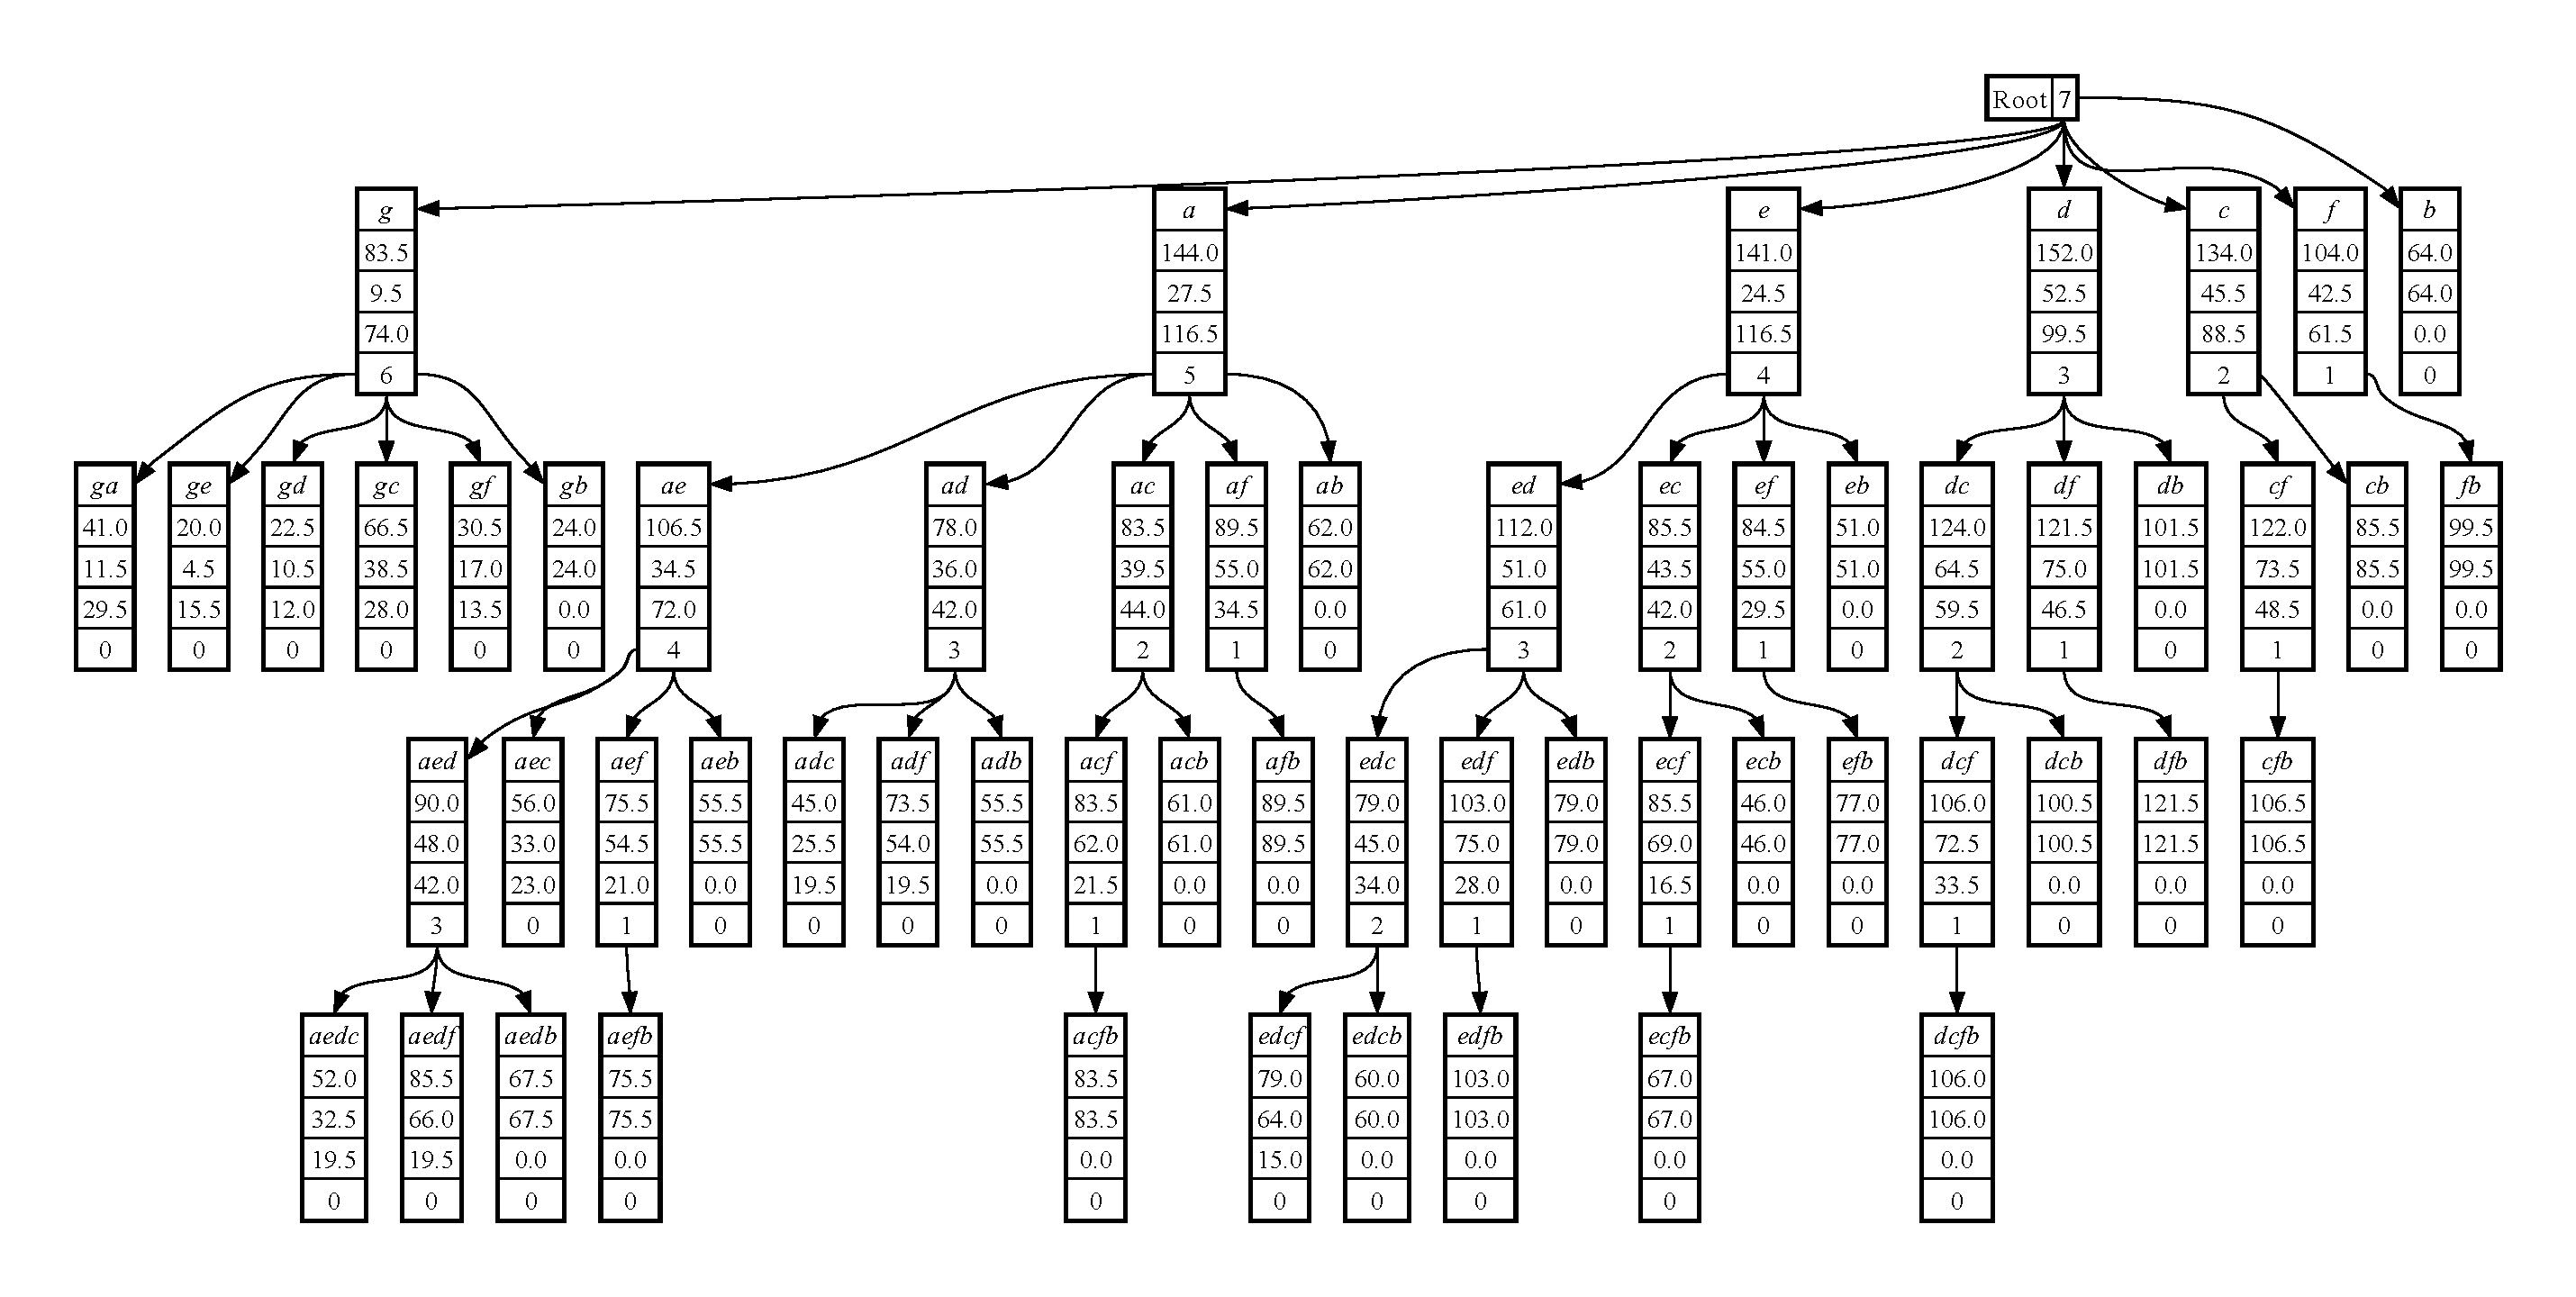
\includegraphics[width=0.95\textwidth]{../Figure/tree.pdf}}
	\caption{This is the tree. }
	\label{fig:tree}
\end{figure*}

\subsection{Discussion}

This is the discussion. This is the discussion. This is the discussion. This is the discussion. This is the discussion. This is the discussion. This is the discussion. This is the discussion. This is the discussion. This is the discussion. 
\section{Conclusion}
\label{sec:6}

This is the conclusion. This is the conclusion. This is the conclusion. This is the conclusion. This is the conclusion. This is the conclusion. This is the conclusion. This is the conclusion. This is the conclusion. This is the conclusion. 

This is the future work. This is the future work. This is the future work. This is the future work. This is the future work. This is the future work. This is the future work. This is the future work. This is the future work. This is the future work. 

\section*{Data Availability}

For the codes and datasets used for accomplishing experiments in this paper, please visit \url{https://github.com/BatchClayderman/onePaperMultipleTypesettingStyles}. 

\section*{Acknowledgement}

Thanks to the editors and the anonymous reviewers for their insightful comments, which improved the quality of this paper. 

\section*{Funding Statement}

There is no funding. 

\section*{Declaration of Competing Interest}

The authors declare that they have no known competing financial interests or personal relationships that could have appeared to influence the work reported in this paper. 

\section*{Authors' Contributions}

All authors reviewed and acknowledged the manuscript. 

\section*{Ethical Consideration Statement}

No human or animal materials are involved in this paper. 
%%%%%%%%%%%%%%%%%%%%%%%%%%%%%%%%%%%%%%%

\bibliographystyle{ACM-Reference-Format}
\bibliography{../Content/ref.bib}

\end{document}
\endinput